\documentclass[12pt,a4paper]{report}

\usepackage{fontspec}
\usepackage[vietnamese]{babel}

\usepackage[a4paper,
top=2.5cm, bottom=2.5cm,
left=3cm,  right=2cm]{geometry}

\usepackage{setspace}
\onehalfspacing
\setlength{\parindent}{1.25cm}

\usepackage{booktabs}
\usepackage{longtable}
\usepackage{float}
\usepackage{amsmath}
\usepackage{hyperref}
\usepackage{algorithm}
\usepackage{algpseudocode}
\usepackage{listings}
\usepackage{xcolor}
\usepackage{array}
\usepackage{tabularx}
\usepackage{graphicx}
\usepackage{amssymb}
\usepackage{multirow}

% ── MÀU SẮC CHO CODE ──────────────────────────────────────────────────────────
\definecolor{codebg}{RGB}{248,248,248}
\definecolor{codeframe}{RGB}{200,200,200}
\definecolor{codekw}{RGB}{0,0,200}        % từ khóa: xanh đậm
\definecolor{codestr}{RGB}{163,21,21}     % chuỗi: đỏ nâu
\definecolor{codecomment}{RGB}{0,128,0}   % comment: xanh lá
\definecolor{codenum}{RGB}{128,128,128}   % số dòng: xám
\definecolor{codebuiltin}{RGB}{0,100,180} % built-in: xanh dương
% ──────────────────────────────────────────────────────────────────────────────

\lstdefinestyle{python}{
  language=Python,
  basicstyle=\ttfamily\footnotesize,
  backgroundcolor=\color{codebg},
  frame=single,
  rulecolor=\color{codeframe},
  breaklines=true,
  keepspaces=true,
  showstringspaces=false,
  numbers=left,
  numberstyle=\tiny\color{codenum},
  tabsize=4,
  keywordstyle=\color{codekw}\bfseries,
  stringstyle=\color{codestr},
  commentstyle=\color{codecomment}\itshape,
  emph={self,None,True,False},
  emphstyle=\color{codebuiltin}\bfseries,
  literate=
    {à}{{\`a}}1 {á}{{\'a}}1 {ả}{{\h{a}}}1 {ã}{{\~a}}1 {ạ}{{\d{a}}}1
    {ă}{{\u{a}}}1 {ắ}{{\'{\u{a}}}}1 {ặ}{{\d{\u{a}}}}1
    {â}{{\^a}}1 {ấ}{{\'{\^a}}}1 {ậ}{{\d{\^a}}}1
    {đ}{{\dj}}1
    {ê}{{\^e}}1 {ề}{{\`{\^e}}}1
    {ô}{{\^o}}1 {ố}{{\'{\^o}}}1 {ộ}{{\d{\^o}}}1
    {ơ}{{\o}}1 {ớ}{{\'{\o}}}1
    {ư}{{\uo}}1 {ứ}{{\'{\uo}}}1
    {ọ}{{\d{o}}}1
}
\lstset{style=python}

\renewcommand{\algorithmicrequire}{\textbf{Đầu vào:}}
\renewcommand{\algorithmicensure}{\textbf{Đầu ra:}}
\floatname{algorithm}{Thuật toán}

\newcommand{\bigO}[1]{$O(#1)$}

% ── THÔNG TIN NHÓM ────────────────────────────────────────────────────────────
\newcommand{\TenDeTai}{Hệ thống quản lý bệnh viện sử dụng hàng đợi ưu tiên}
\newcommand{\TenMon}{Cấu trúc dữ liệu và Giải thuật}
\newcommand{\GiaoVien}{Vương Mai Phương}
\newcommand{\ThanhVienA}{Đặng Tuấn Đạt -- 202418867}
\newcommand{\ThanhVienB}{Nguyễn Mai Đức -- 202418870}
\newcommand{\ThanhVienC}{Nguyễn Huy Đức -- 202418871}
\newcommand{\ThanhVienD}{Nguyễn Bá Dũng -- 202418877}
\newcommand{\ThanhVienE}{Nguyễn Hải Dương -- 20227102}
% ──────────────────────────────────────────────────────────────────────────────

\begin{document}

% ═════════════════════════════════════════════════════════════════════════════
%  TRANG BÌA
% ═════════════════════════════════════════════════════════════════════════════
\begin{titlepage}
\centering
{\large\bfseries ĐẠI HỌC BÁCH KHOA HÀ NỘI}\\[0.3cm]
{\large\bfseries KHOA TOÁN -- TIN}\\[1.5cm]

\IfFileExists{logoBK.png}{%
  
\includegraphics[width=3.6cm]{logoBK.png}\\[1cm]%
}{%
  \fbox{\parbox[c][3.6cm][c]{3.6cm}{\centering\textbf{LOGO\\BÁCH KHOA}}}\\[1cm]%
}

{\large Báo cáo Bài tập lớn cuối kỳ}\\[0.4cm]
{\LARGE\bfseries \TenMon}\\[0.8cm]
{\Large\bfseries \TenDeTai}\\[1.5cm]

{\normalsize GVHD: \GiaoVien}\\[0.4cm]
{\normalsize Nhóm 9}\\[0.8cm]

\begin{tabular}{c}
\ThanhVienA \\
\ThanhVienB \\
\ThanhVienC \\
\ThanhVienD \\
\ThanhVienE \\
\end{tabular}\\[2cm]

{\normalsize Hà Nội, tháng 6 năm \the\year}
\end{titlepage}

\tableofcontents
\listoftables

% ═════════════════════════════════════════════════════════════════════════════
\chapter*{Lời mở đầu}
\addcontentsline{toc}{chapter}{Lời mở đầu}
% ═════════════════════════════════════════════════════════════════════════════

Đề tài \textit{\TenDeTai} được lựa chọn dựa trên mục đích xây dựng hệ thống quản lý và phân loại bệnh nhân bằng cấu trúc hàng đợi ưu tiên, vốn được thực hiện thủ công dẫn đến dễ sai sót và khó bảo trì

Mục tiêu của bài toán là xây dựng chương trình có khả năng thêm bệnh nhân,
gọi bệnh nhân ưu tiên nhất vào khám, tìm kiếm, sửa, xóa thông tin và lưu
lịch sử khám. Nhóm tiếp cận bài toán bằng cách phân tích chức năng, thiết
kế cấu trúc dữ liệu, sau đó triển khai bằng ngôn ngữ lập trình Python.

Báo cáo được tổ chức thành các chương: Chương~\ref{ch:phan-tich} phân tích
bài toán; Chương~\ref{ch:thiet-ke} trình bày thiết kế hệ thống và cài đặt
chương trình; Chương~\ref{ch:giao-dien} giới thiệu giao diện người dùng;
Chương~\ref{ch:thu-nghiem} trình bày kết quả thực nghiệm;
Chương~\ref{ch:kiem-thu} trình bày kiểm thử; Chương~\ref{ch:ket-luan}
kết luận và hướng phát triển.

% ═════════════════════════════════════════════════════════════════════════════
\chapter{Phân tích bài toán}
\label{ch:phan-tich}
% ═════════════════════════════════════════════════════════════════════════════

Bài toán đặt ra là thiết kế và triển khai một hệ thống quản lý hàng đợi bệnh nhân của một bệnh viên. Hệ thống cần giải quyết được các vấn đề như số lượng bệnh nhân khổng lồ, đảm bảo ưu tiên bệnh nhân nguy kịch đồng thời duy trì tính công bằng giữa các bệnh nhân có cùng mức độ ưu tiên

\section{Bối cảnh thực tế}

Tại các phòng cấp cứu và phòng khám bệnh viện, số lượng bệnh nhân đến khám
mỗi ngày thường rất lớn và không đến theo thứ tự mức độ nguy hiểm. Thực tế
cho thấy một bệnh nhân bị đau tim có thể đến sau một bệnh nhân chỉ bị cảm
nhẹ -- nếu áp dụng FIFO (đến trước khám trước) thì bệnh nhân nguy kịch vẫn
phải chờ, gây nguy hiểm đến tính mạng.

Hệ thống cần xây dựng là một phần mềm có khả năng:
\begin{itemize}
  \item Tự động xếp thứ tự bệnh nhân theo mức độ ưu tiên y tế.
  \item Đảm bảo người nguy kịch luôn được khám trước.
  \item Duy trì tính công bằng FIFO khi hai bệnh nhân có cùng mức độ bệnh
        (ai đến trước thì được khám trước).
\end{itemize}

Đây là bài toán điển hình của Priority Queue (hàng đợi ưu tiên) trong khoa
học máy tính, ứng dụng thực tiễn vào lĩnh vực y tế.

\section{Yêu cầu chức năng}

\begin{enumerate}
  \item \textbf{Quản lý hàng đợi bệnh nhân:}
        \begin{itemize}
          \item Lưu trữ thông tin mỗi bệnh nhân gồm: mã số (tự động sinh tăng
                dần), họ tên, tuổi, mức độ bệnh (1--5), giờ đến.
          \item Cho phép cập nhật thông tin khi có sai sót (ví dụ: nhập nhầm
                mức độ bệnh ban đầu).
          \item Cho phép xóa bệnh nhân khỏi hàng đợi (ví dụ: bệnh nhân tự về
                hoặc chuyển viện trước khi được khám).
          \item Hỗ trợ tìm kiếm theo mã số hoặc theo tên bệnh nhân.
        \end{itemize}

  \item \textbf{Gọi bệnh nhân vào khám:}
        Lấy bệnh nhân ưu tiên nhất khỏi hàng đợi. Quy tắc ưu tiên 3 cấp:
        \begin{itemize}
          \item Cấp 1: Mức độ bệnh nhỏ hơn $\Rightarrow$ ưu tiên hơn
                (1 = nguy kịch, 2 = nặng, 3 = trung bình, 4 = nhẹ,
                5 = rất nhẹ).
          \item Cấp 2: Nếu cùng mức độ $\Rightarrow$ người đến sớm hơn
                $\Rightarrow$ ưu tiên hơn (đảm bảo tính công bằng FIFO).
          \item Cấp 3: Nếu cùng cả mức độ lẫn giờ đến $\Rightarrow$ số đăng
                ký nhỏ hơn $\Rightarrow$ ưu tiên hơn (tie-breaker).
        \end{itemize}
        Bệnh nhân sau khi được gọi sẽ bị xóa khỏi hàng đợi và chuyển sang
        danh sách lịch sử.

  \item \textbf{Quản lý lịch sử khám:}
        \begin{itemize}
          \item Ghi lại toàn bộ bệnh nhân đã khám theo đúng thứ tự thời gian
                thực tế được gọi vào phòng khám.
          \item Lịch sử giúp tra cứu lại ca khám, phục vụ kiểm tra hoặc báo
                cáo cuối ngày.
        \end{itemize}

  \item \textbf{Thống kê:}
        \begin{itemize}
          \item Báo cáo tổng số bệnh nhân đang chờ và đã khám.
          \item Phân loại theo từng mức độ bệnh (1--5) để ban quản lý nắm
                được tình hình tổng thể của phòng khám.
        \end{itemize}

  \item \textbf{Lưu trữ dữ liệu (\texttt{loadData} / \texttt{saveData}):}
        \begin{itemize}
          \item Sau mỗi thao tác thay đổi dữ liệu, hệ thống tự động ghi
                xuống file CSV.
          \item Khi khởi động lại chương trình, dữ liệu được đọc từ file và
                khôi phục nguyên vẹn hàng đợi và lịch sử.
          \item Mục đích: đảm bảo không mất dữ liệu khi tắt chương trình
                đột ngột (mất điện, lỗi hệ thống\ldots).
        \end{itemize}
\end{enumerate}

\section{Yêu cầu phi chức năng}

Ngoài các chức năng trên, hệ thống còn phải đáp ứng các tiêu chí kỹ thuật sau:

\begin{itemize}
  \item \textbf{Hiệu suất:} Các thao tác cốt lõi (thêm bệnh nhân, gọi khám)
        phải có độ phức tạp thời gian $O(\log N)$, đảm bảo phản hồi nhanh ngay
        cả khi hàng đợi chứa hàng nghìn bệnh nhân. Với $N = 10.000$, mỗi thao
        tác chỉ mất khoảng 13 bước tính toán thay vì 10.000 bước như danh sách
        thông thường.
  \item \textbf{Độ tin cậy:} Dữ liệu không được mất sau khi tắt chương trình.
        Mọi thay đổi phải được ghi xuống file ngay lập tức, không chờ đến khi
        thoát.
  \item \textbf{Khả năng mở rộng:} Kiến trúc được tổ chức thành các lớp riêng
        biệt, tách biệt dữ liệu, logic xử lý và giao diện người dùng. Nhờ đó có
        thể dễ dàng bổ sung tính năng mới mà không phải viết lại toàn bộ chương
        trình.
\end{itemize}

\section{Phát biểu bài toán}

\textbf{Đầu vào:}
\begin{itemize}
  \item Danh sách bệnh nhân đến khám, mỗi người gồm: họ tên, tuổi, mức độ
        bệnh (1--5), giờ đến (định dạng \texttt{HH:MM}).
  \item Các thao tác người dùng thực hiện: thêm bệnh nhân, gọi khám, sửa
        thông tin, xóa, tìm kiếm.
\end{itemize}

\textbf{Đầu ra:}
\begin{itemize}
  \item Mỗi lần gọi khám, hệ thống trả về đúng bệnh nhân có độ ưu tiên cao
        nhất theo quy tắc 3 cấp.
  \item Lịch sử khám được lưu đầy đủ và có thể truy xuất lại.
  \item Toàn bộ dữ liệu được lưu xuống file sau mỗi thay đổi, không mất khi
        tắt chương trình.
\end{itemize}

\textbf{Ràng buộc:}
\begin{itemize}
  \item Mức độ bệnh là số nguyên từ 1 đến 5, số càng nhỏ thì mức độ ưu tiên
        càng cao (1 = nguy kịch, 5 = rất nhẹ).
  \item Khi hai bệnh nhân có cùng mức độ bệnh, người đến sớm hơn được ưu tiên
        (FIFO).
  \item Khi cùng cả mức độ lẫn giờ đến, dùng số thứ tự đăng ký nhỏ hơn làm
        tie-breaker để đảm bảo hệ thống luôn có kết quả xác định.
\end{itemize}

\section{Lý do không dùng danh sách thông thường}

Khi xây dựng hàng đợi ưu tiên, hai cách tiếp cận đơn giản nhất là dùng danh
sách chưa sắp xếp hoặc danh sách đã sắp xếp. Tuy nhiên cả hai đều có điểm
yếu rõ ràng:

\begin{itemize}
  \item \textbf{Unsorted List:} Thêm mới \bigO{1} nhưng mỗi lần gọi khám
        phải duyệt toàn bộ để tìm người ưu tiên nhất -- \bigO{N}. Với 10.000
        bệnh nhân, mỗi lần bác sĩ nhấn ``gọi khám'' hệ thống phải duyệt
        10.000 bản ghi.
  \item \textbf{Sorted List:} Gọi khám \bigO{1} nhưng thêm mới phải tìm vị
        trí đúng và dịch mảng -- \bigO{N}. Mỗi lần có bệnh nhân mới đăng ký,
        hệ thống phải sắp xếp lại toàn bộ.
\end{itemize}

\textbf{Binary Min-Heap} giải quyết cả hai: thêm mới \bigO{\log N}, lấy phần
tử ưu tiên nhất \bigO{\log N}. Heap được lưu dưới dạng mảng, với nút tại vị
trí $i$:
\[
  \text{cha}(i) = \left\lfloor\frac{i-1}{2}\right\rfloor, \quad
  \text{con trái} = 2i+1, \quad
  \text{con phải} = 2i+2
\]

\begin{table}[H]
\centering
\caption{So sánh các cấu trúc dữ liệu cho bài toán hàng đợi ưu tiên}
\begin{tabular}{llll}
\toprule
\textbf{Tiêu chí} & \textbf{Unsorted List} & \textbf{Sorted List} & \textbf{Binary Min-Heap} \\
\midrule
Thêm bệnh nhân        & \bigO{1}      & \bigO{N}      & \bigO{\log N} \\
Gọi khám              & \bigO{N}      & \bigO{1}      & \bigO{\log N} \\
$N = 10.000$ (worst)  & 10.000 bước  & 10.000 bước  & $\sim$13 bước $\checkmark$ \\
Bộ nhớ                & \bigO{N}      & \bigO{N}      & \bigO{N} \\
Phù hợp bài toán      & Không         & Không         & Có $\checkmark$ \\
\bottomrule
\end{tabular}
\end{table}

% ═════════════════════════════════════════════════════════════════════════════
\chapter{Thiết kế hệ thống và cài đặt chương trình}
\label{ch:thiet-ke}
% ═════════════════════════════════════════════════════════════════════════════

\section{Kiến trúc tổng thể và phân chia module}

Hệ thống được tổ chức thành bốn tầng tách biệt. Mỗi tầng chỉ giao tiếp với
tầng ngay dưới, không truy cập trực tiếp vào thuộc tính nội bộ của tầng khác.

\begin{table}[H]
\centering
\caption{Cấu trúc thư mục và vai trò module}
\begin{tabular}{p{2.8cm}p{6.5cm}p{6cm}}
\toprule
\textbf{Tầng} & \textbf{Module / File} & \textbf{Vai trò} \\
\midrule
Data           & \texttt{Data/patient.py}
               & Kiểu dữ liệu \texttt{Patient}, quy tắc so sánh ưu tiên \\
DataStructures & \texttt{DataStructures/min\_heap.py}
               & ADT Min-Heap tự cài đặt \\
               & \texttt{DataStructures/linked\_list.py}
               & ADT Linked List đơn \\
               & \texttt{DataStructures/hash\_map.py}
               & ADT HashMap (bảng băm) \\
Algorithm      & \texttt{Algorithm/priority\_queue.py}
               & Hàng đợi ưu tiên bệnh nhân dùng MinHeap \\
               & \texttt{Algorithm/history\_tracker.py}
               & Lịch sử khám dùng LinkedList \\
               & \texttt{Algorithm/scheduler.py}
               & Điều phối toàn bộ nghiệp vụ \\
UI             & \texttt{UI/main\_console.py}
               & Giao diện console người dùng \\
\bottomrule
\end{tabular}
\end{table}
\clearpage
\section{Sơ đồ lớp (Class Diagram)}

\begin{figure}[H]
\centering
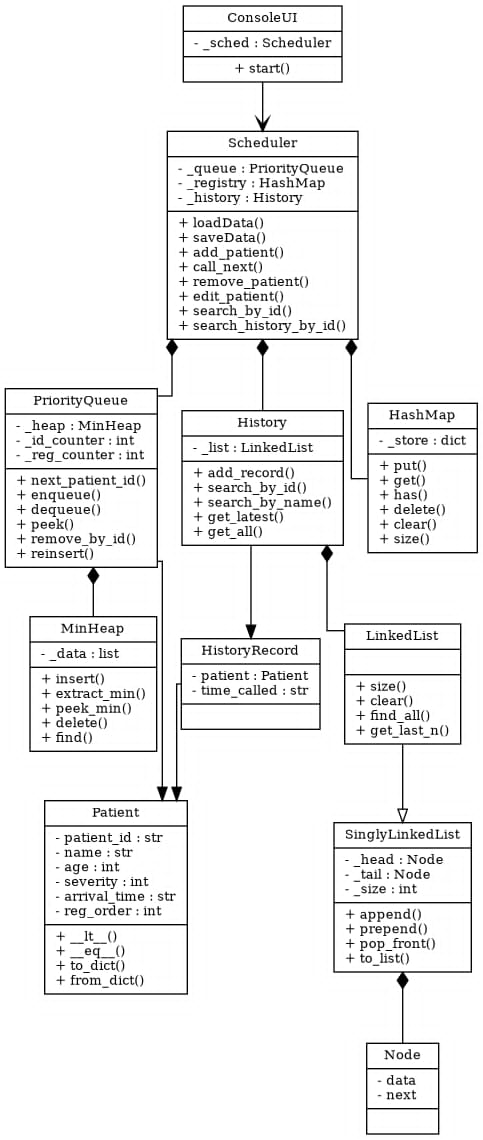
\includegraphics[width=0.5\textwidth]{cld.png}
\caption{Sơ đồ lớp hệ thống quản lý bệnh viện}
\label{fig:class-diagram}
\end{figure}

\clearpage

\section{Cấu trúc dữ liệu}

Mục này trình bày cài đặt bốn thành phần cốt lõi theo thứ tự phân tầng từ
dưới lên: \texttt{Patient} (tầng Data), \texttt{MinHeap},
\texttt{SinglyLinkedList} và \texttt{PatientHashMap} (tầng DataStructures).

\subsection{Lớp Patient -- kiểu dữ liệu và quy tắc so sánh ưu tiên}

\texttt{MinHeap} không biết tới ''patient'' -- nó chỉ gọi toán tử
so sánh; \texttt{Patient} tự định nghĩa toán tử đó để quyết định thứ tự
ưu tiên.

\begin{lstlisting}[caption=Khởi tạo và quy tắc so sánh ưu tiên 3 cấp (patient.py)]
class Patient:
    def __init__(self, patient_id, name, age, severity,
                 arrival_time, reg_order=0):
        self.patient_id   = str(patient_id).strip()
        self.name         = str(name).strip()
        self.age          = int(age)
        self.severity     = int(severity)
        self.arrival_time = str(arrival_time).strip()
        self.reg_order    = int(reg_order)

    def __lt__(self, other):
        if self.severity != other.severity:
            return self.severity < other.severity       # cap 1
        if self.arrival_time != other.arrival_time:
            return self.arrival_time < other.arrival_time  # cap 2
        return self.reg_order < other.reg_order         # cap 3
\end{lstlisting}

Ba cấp ưu tiên: (1) \textbf{severity} -- số càng nhỏ càng nặng; (2)
\textbf{arrival\_time} -- cùng mức độ thì đến trước khám trước (FIFO); (3)
\textbf{reg\_order} -- số thứ tự đăng ký, không reset khi khởi động
lại, đảm bảo luôn so sánh được.
\newpage
\texttt{arrival\_time} được so sánh như chuỗi khi format đồng nhất
\texttt{HH:MM}. Hàm \\\texttt{validate\_arrival\_time()} tự động chuẩn hoá
\texttt{"9:00"} thành \texttt{"09:00"}:

\begin{lstlisting}[caption=Tự động chuẩn hoá định dạng giờ (patient.py)]
_TIME_RE = re.compile(r'^([01]\d|2[0-3]):[0-5]\d$')

def validate_arrival_time(time_str: str) -> tuple[bool, str]:
    s = str(time_str).strip()
    if _TIME_RE.match(s):
        return True, s
    if re.match(r'^\d:[0-5]\d$', s):
        fixed = '0' + s
        if _TIME_RE.match(fixed):
            return True, fixed
    return False, f"Gio den '{time_str}' khong hop le."
\end{lstlisting}

\begin{table}[H]
\centering
\caption{Thuộc tính lớp \texttt{Patient}}
\begin{tabular}{lll}
\toprule
\textbf{Thuộc tính} & \textbf{Kiểu} & \textbf{Mô tả} \\
\midrule
\texttt{patient\_id}   & str & Mã tự động, ví dụ \texttt{BN0001} \\
\texttt{name}          & str & Họ và tên \\
\texttt{age}           & int & Tuổi \\
\texttt{severity}      & int & Mức độ bệnh 1 (nguy kịch) -- 5 (rất nhẹ) \\
\texttt{arrival\_time} & str & Giờ đến, định dạng \texttt{HH:MM} \\
\texttt{reg\_order}    & int & Số thứ tự đăng ký, dùng làm tie-breaker \\
\bottomrule
\end{tabular}
\end{table}

\subsection{ADT MinHeap -- hàng đợi ưu tiên lõi}

\texttt{MinHeap} là cấu trúc thuần túy -- toàn bộ dữ liệu nằm trong mảng
\texttt{\_data}, quan hệ cha-con tính bằng chỉ số, không dùng con trỏ.

\begin{lstlisting}[caption=insert và \_heapify\_up: O(log N) (min\_heap.py)]
def insert(self, item):
    self._data.append(item)
    self._heapify_up(len(self._data) - 1)

def _heapify_up(self, i):
    parent = (i - 1) // 2
    if i > 0 and self._data[i] < self._data[parent]:
        self._data[i], self._data[parent] = \
            self._data[parent], self._data[i]
        self._heapify_up(parent)
\end{lstlisting}

Mỗi bước chỉ số $i$ được chia đôi để lên cha; tối đa $\lfloor\log_2 N\rfloor$
bước $\Rightarrow$ \textbf{\bigO{\log N}}.

\begin{lstlisting}[caption=extract\_min và \_heapify\_down: O(log N) (min\_heap.py)]
def extract_min(self):
    if self.is_empty(): return None
    if len(self._data) == 1: return self._data.pop()
    minimum = self._data[0]
    self._data[0] = self._data.pop()  # tranh pop(0) O(N)
    self._heapify_down(0)
    return minimum

def _heapify_down(self, i):
    smallest, n = i, len(self._data)
    left, right = 2*i + 1, 2*i + 2
    if left  < n and self._data[left]  < self._data[smallest]:
        smallest = left
    if right < n and self._data[right] < self._data[smallest]:
        smallest = right
    if smallest != i:
        self._data[i], self._data[smallest] = \
            self._data[smallest], self._data[i]
        self._heapify_down(smallest)
\end{lstlisting}

Thao tác \texttt{delete} theo predicate tìm vị trí \bigO{N}, sau đó đổi chỗ
với phần tử cuối và gọi cả \texttt{\_heapify\_up} lẫn \texttt{\_heapify\_down}
để phục hồi heap:

\begin{lstlisting}[caption=delete theo predicate (min\_heap.py)]
def delete(self, predicate):
    idx = next((i for i, x in enumerate(self._data)
                if predicate(x)), -1)
    if idx == -1: return None
    removed = self._data[idx]
    if idx == len(self._data) - 1:
        self._data.pop()
    else:
        self._data[idx] = self._data.pop()
        self._heapify_up(idx)
        self._heapify_down(idx)
    return removed
\end{lstlisting}

\begin{table}[H]
\centering
\caption{Các phương thức \texttt{MinHeap} và độ phức tạp}
\begin{tabular}{p{3.8cm}p{5.7cm}p{1.8cm}}
\toprule
\textbf{Phương thức} & \textbf{Mô tả} & \textbf{Big O} \\
\midrule
\texttt{insert(item)}          & Thêm vào cuối + \texttt{\_heapify\_up}            & \bigO{\log N} \\
\texttt{extract\_min()}        & Lấy đỉnh, đưa cuối lên + \texttt{\_heapify\_down} & \bigO{\log N} \\
\texttt{peek\_min()}           & Trả về \texttt{data[0]}, không xóa                & \bigO{1}      \\
\texttt{delete(predicate)}     & Tìm tuyến tính + xóa + sửa heap                   & \bigO{N}      \\
\texttt{find(predicate)}       & Duyệt toàn bộ mảng                                & \bigO{N}      \\
\texttt{to\_sorted\_list()}    & Sao chép + sắp xếp                                & \bigO{N\log N}\\
\texttt{is\_empty()}, \texttt{size()} & Truy cập trực tiếp                       & \bigO{1}      \\
\texttt{\_heapify\_up(i)}      & Đẩy lên tối đa $\log N$ tầng                      & \bigO{\log N} \\
\texttt{\_heapify\_down(i)}    & Đẩy xuống tối đa $\log N$ tầng                    & \bigO{\log N} \\
\bottomrule
\end{tabular}
\end{table}

\subsection{ADT SinglyLinkedList -- lưu lịch sử khám}

Lịch sử khám chỉ cần \textit{append} \bigO{1} và \textit{duyệt tuần tự}
\bigO{N}. Con trỏ \texttt{\_tail} riêng biệt là điểm mấu chốt --
\texttt{append} không phải duyệt đến cuối:

\begin{lstlisting}[caption=Node và append O(1) nhờ con trỏ \_tail (linked\_list.py)]
class Node:
    __slots__ = ('data', 'next')
    def __init__(self, data):
        self.data = data; self.next = None

class SinglyLinkedList:
    def __init__(self):
        self._head = self._tail = None
        self._size = 0

    def append(self, data) -> None:
        new_node = Node(data)
        if self._tail is None:
            self._head = self._tail = new_node
        else:
            self._tail.next = new_node
            self._tail = new_node
        self._size += 1
\end{lstlisting}

\begin{table}[H]
\centering
\caption{Các phương thức \texttt{SinglyLinkedList} và độ phức tạp}
\begin{tabular}{p{3.5cm}p{6cm}p{1.8cm}}
\toprule
\textbf{Phương thức} & \textbf{Mô tả} & \textbf{Big O} \\
\midrule
\texttt{append(data)}   & Thêm vào cuối, nhờ con trỏ \texttt{tail} & \bigO{1} \\
\texttt{prepend(data)}  & Thêm vào đầu, cập nhật \texttt{head}     & \bigO{1} \\
\texttt{find\_first(p)} & Duyệt từ head, trả về kết quả đầu tiên  & \bigO{N} \\
\texttt{find\_all(p)}   & Duyệt toàn bộ, trả về list kết quả      & \bigO{N} \\
\texttt{to\_list()}     & Duyệt từ head đến tail                   & \bigO{N} \\
\texttt{size()}, \texttt{is\_empty()} & Truy cập biến \texttt{\_size} & \bigO{1} \\
\texttt{clear()}        & Đặt head, tail = None; \_size = 0        & \bigO{1} \\
\bottomrule
\end{tabular}
\end{table}

\subsection{ADT PatientHashMap -- registry tra cứu nhanh}

\texttt{MinHeap} không hỗ trợ random access theo ID (\bigO{N} để tìm).
\texttt{PatientHashMap} giải quyết bằng cơ chế băm:
\texttt{hash("BN0042")} $\rightarrow$ chỉ số slot $\rightarrow$ \textbf{\bigO{1}}.

Lớp duy trì song song: \texttt{\_store} (dict CPython) cho production path,
và \texttt{\_demo} (\texttt{\_ChainHashMap} tự cài đặt Separate Chaining) để
minh họa cơ chế:

\begin{mini}
\begin{lstlisting}[caption=Separate Chaining và rehash trong \_ChainHashMap (hash\_map.py)]
class _ChainHashMap:
    _LOAD_MAX = 0.75

    def _index(self, key: str) -> int:
        return abs(hash(key)) % self._cap

    def put(self, key: str, value) -> None:
        idx = self._index(key)
        bucket = self._table[idx]
        for i, (k, _) in enumerate(bucket):
            if k == key:
                bucket[i] = (key, value); return
        bucket.append((key, value))
        self._size += 1
        if self._size / self._cap > self._LOAD_MAX:
            self._rehash()

    def _rehash(self) -> None:          # O(N), hiem gap
        old_table = self._table
        self._cap *= 2
        self._table = [[] for _ in range(self._cap)]
        self._size = 0
        for bucket in old_table:
            for key, value in bucket:
                self.put(key, value)
\end{lstlisting}

Khi load factor $\alpha > 0{,}75$, \texttt{\_rehash} nhân đôi mảng và băm lại
toàn bộ -- \bigO{N} mỗi lần nhưng ngày càng ít xảy ra $\Rightarrow$
\textit{amortised} \bigO{1} cho mỗi \texttt{put}.

\begin{lstlisting}[caption={register, lookup, unregister trong PatientHashMap (hash\_map.py)}]
class PatientHashMap:
    def __init__(self):
        self._store: dict = {}
        self._demo = _ChainHashMap(16)

    def register(self, patient) -> None:
        if not hasattr(patient, 'patient_id'):
            raise TypeError(
                f"Chi nhan Patient; nhan {type(patient).__name__}.")
        self._store[patient.patient_id] = patient
        self._demo.put(patient.patient_id, patient)

    def lookup(self, patient_id: str):
        return self._store.get(patient_id)

    def unregister(self, patient_id: str) -> bool:
        if patient_id in self._store:
            del self._store[patient_id]
            self._demo.delete(patient_id)
            return True
        return False
\end{lstlisting}

\textbf{Phối hợp MinHeap và PatientHashMap:} Khi thêm bệnh nhân, cả hai đều
cập nhật đồng thời. Khi sửa/xóa, Scheduler tra map trước \bigO{1} rồi mới gọi
\texttt{heap.delete()} \bigO{N}. Nhờ vậy, không thao tác nào trên đường chính
(thêm, gọi khám) vượt quá \bigO{\log N}.

\begin{table}[H]
\centering
\caption{Các phương thức \texttt{PatientHashMap} và độ phức tạp}
\begin{tabular}{p{3.5cm}p{6cm}p{1.8cm}}
\toprule
\textbf{Phương thức} & \textbf{Mô tả} & \textbf{Big O} \\
\midrule
\texttt{register(patient)} & Lưu hoặc ghi đè cặp (key, value)   & \bigO{1}$^*$ \\
\texttt{lookup(key)}       & Tra cứu theo key                    & \bigO{1}$^*$ \\
\texttt{unregister(key)}   & Xóa cặp (key, value)               & \bigO{1}$^*$ \\
\texttt{size()}, \texttt{is\_empty()} & Số cặp hiện có         & \bigO{1}   \\
\bottomrule
\multicolumn{3}{l}{\footnotesize $^*$ Trung bình. Trường hợp xấu nhất \bigO{N} khi nhiều va chạm hash.}
\end{tabular}
\end{table}

\section{Giả mã các thuật toán}

\subsection{loadData -- Đọc dữ liệu từ file}

\begin{algorithm}[H]
\caption{loadData()}
\begin{algorithmic}[1]
\Require File \texttt{queue.csv} và \texttt{history.csv}
\Ensure Hàng đợi và lịch sử được nạp vào bộ nhớ
\State Mở file \texttt{queue.csv}
\If{file không tồn tại}
  \State Kết thúc (hàng đợi bắt đầu rỗng)
\EndIf
\For{mỗi dòng trong file}
  \State Phân tích dòng CSV thành các trường dữ liệu
  \State Tạo đối tượng \texttt{Patient} từ các trường đó
  \State \Call{MinHeap.insert}{Patient}
\EndFor
\State Xây dựng lại registry: duyệt heap, \Call{HashMap.put}{id, Patient}
\State Đọc \texttt{history.csv} tương tự, \Call{LinkedList.append}{HistoryRecord}
\end{algorithmic}
\end{algorithm}

\subsection{saveData -- Ghi dữ liệu xuống file}

\begin{algorithm}[H]
\caption{saveData()}
\begin{algorithmic}[1]
\Require Hàng đợi và lịch sử hiện có trong bộ nhớ
\Ensure Dữ liệu được ghi ra \texttt{queue.csv} và \texttt{history.csv}
\State Mở file \texttt{queue.csv} để ghi (ghi đè)
\State Ghi dòng tiêu đề CSV
\For{mỗi \texttt{Patient} trong mảng nội bộ của MinHeap}
  \State Ghi dòng: id, tên, tuổi, mức độ, giờ đến, số đăng ký
\EndFor
\State Mở file \texttt{history.csv} để ghi (ghi đè), ghi toàn bộ lịch sử
\end{algorithmic}
\end{algorithm}

\subsection{Thêm bệnh nhân -- enqueue / heapify\_up}

\begin{algorithm}[H]
\caption{addPatient(name, age, severity, arrival\_time)}
\begin{algorithmic}[1]
\Require Thông tin bệnh nhân mới
\Ensure Bệnh nhân được thêm vào hàng đợi, dữ liệu được lưu
\If{thông tin không hợp lệ}
  \State Thông báo lỗi, kết thúc
\EndIf
\State $id \gets$ sinh ID tự động dạng \texttt{BNxxxx}
\State $reg \gets$ tăng bộ đếm thứ tự đăng ký
\State Tạo đối tượng \texttt{Patient(id, name, age, severity, arrival\_time, reg)}
\State \Call{MinHeap.insert}{Patient}
\State \Call{HashMap.put}{id, Patient}
\State \Call{saveData}{}
\end{algorithmic}
\end{algorithm}

\begin{algorithm}[H]
\caption{heapify\_up(i)}
\begin{algorithmic}[1]
\Require $i$: vị trí phần tử vừa thêm (cuối mảng)
\State $parent \gets \lfloor(i-1)/2\rfloor$
\If{$i > 0$ \textbf{và} $data[i] < data[parent]$}
  \State Đổi chỗ $data[i]$ và $data[parent]$
  \State \Call{heapify\_up}{$parent$}
\EndIf
\end{algorithmic}
\end{algorithm}

\noindent\textbf{Độ phức tạp:} \bigO{\log N} -- cây có chiều cao
$\lfloor\log_2 N\rfloor$, heapify\_up đi lên tối đa bấy nhiêu tầng.

\subsection{Gọi bệnh nhân vào khám -- dequeue / heapify\_down}

\begin{algorithm}[H]
\caption{callNext()}
\begin{algorithmic}[1]
\Ensure Trả về bệnh nhân ưu tiên nhất; cập nhật lịch sử và file
\If{hàng đợi rỗng}
  \State Thông báo ``không có bệnh nhân'', kết thúc
\EndIf
\State $p \gets$ \Call{MinHeap.extract\_min}{}
\State \Call{HashMap.delete}{$p$.id}
\State \Call{LinkedList.append}{HistoryRecord($p$, giờ hiện tại)}
\State \Call{saveData}{}
\State \Return $p$
\end{algorithmic}
\end{algorithm}

\begin{algorithm}[H]
\caption{heapify\_down(i)}
\begin{algorithmic}[1]
\Require $i$: vị trí cần đẩy xuống; $N$: số phần tử
\State $smallest \gets i$; \quad $left \gets 2i+1$; \quad $right \gets 2i+2$
\If{$left < N$ \textbf{và} $data[left] < data[smallest]$}
  \State $smallest \gets left$
\EndIf
\If{$right < N$ \textbf{và} $data[right] < data[smallest]$}
  \State $smallest \gets right$
\EndIf
\If{$smallest \neq i$}
  \State Đổi chỗ $data[i]$ và $data[smallest]$
  \State \Call{heapify\_down}{$smallest$}
\EndIf
\end{algorithmic}
\end{algorithm}

\noindent\textbf{Độ phức tạp:} \bigO{\log N} -- tương tự heapify\_up, đi
xuống tối đa $\log N$ tầng.

\subsection{Tìm kiếm và xóa bệnh nhân}

\begin{algorithm}[H]
\caption{searchById(id)}
\begin{algorithmic}[1]
\State \Return \Call{HashMap.get}{id} \Comment{\bigO{1} trung bình}
\end{algorithmic}
\end{algorithm}

\begin{algorithm}[H]
\caption{removePatient(id)}
\begin{algorithmic}[1]
\If{\textbf{không} \Call{HashMap.has}{id}}
  \State Thông báo ``không tìm thấy'', kết thúc
\EndIf
\State Duyệt mảng heap, tìm vị trí $i$ có $data[i]$.id $=$ id \Comment{\bigO{N}}
\State Đổi $data[i]$ với phần tử cuối, xóa phần tử cuối
\State \Call{heapify\_up}{$i$}; \quad \Call{heapify\_down}{$i$}
\State \Call{HashMap.delete}{id}
\State \Call{saveData}{}
\end{algorithmic}
\end{algorithm}

\section{Phân tích độ phức tạp}

\subsection{Độ phức tạp thời gian}

\begin{table}[H]
\centering
\caption{Bảng tổng hợp độ phức tạp thời gian}
\begin{tabular}{llll}
\toprule
\textbf{Thao tác} & \textbf{Cấu trúc} & \textbf{Thời gian} & \textbf{Giải thích} \\
\midrule
Thêm bệnh nhân   & MinHeap    & \bigO{\log N}  & Heapify up theo chiều cao cây \\
Gọi khám         & MinHeap    & \bigO{\log N}  & Heapify down theo chiều cao cây \\
Xem tiếp theo    & MinHeap    & \bigO{1}       & Luôn ở \texttt{data[0]} \\
Tìm theo ID      & HashMap    & \bigO{1}       & Tra cứu trực tiếp qua mã băm \\
Xóa/Sửa thông tin & MinHeap  & \bigO{N}       & Duyệt mảng tìm vị trí phần tử \\
Lưu lịch sử      & LinkedList & \bigO{1}       & Sử dụng con trỏ \textit{tail} \\
loadData         & --         & \bigO{N\log N} & Đọc $N$ dòng, mỗi dòng enqueue \bigO{\log N} \\
saveData         & --         & \bigO{N}       & Duyệt toàn bộ, ghi từng dòng \\
\bottomrule
\end{tabular}
\end{table}

\subsection{Độ phức tạp không gian}

\begin{table}[H]
\centering
\caption{Bảng tổng hợp độ phức tạp không gian}
\begin{tabular}{lll}
\toprule
\textbf{Cấu trúc} & \textbf{Không gian} & \textbf{Giải thích} \\
\midrule
MinHeap (hàng đợi)       & \bigO{N}       & Mảng $N$ phần tử \\
HashMap (registry)       & \bigO{N}       & $N$ cặp (key, Patient) \\
LinkedList (lịch sử)     & \bigO{M}       & $M$ = số lượt đã khám \\
heapify\_up/down (stack) & \bigO{\log N}  & Đệ quy sâu tối đa $\log N$ tầng \\
\bottomrule
\end{tabular}
\end{table}

% ═════════════════════════════════════════════════════════════════════════════
\chapter{Giao diện người dùng}
\label{ch:giao-dien}
% ═════════════════════════════════════════════════════════════════════════════

\section{Tổng quan thiết kế giao diện}

Hệ thống sử dụng giao diện dòng lệnh (Console UI), triển khai toàn bộ trong
file \texttt{UI/main\_console.py}. Lớp \texttt{ConsoleUI} \textbf{chỉ} giao
tiếp với \texttt{Scheduler} -- tuyệt đối không truy cập trực tiếp vào heap,
linked list hay bất kỳ cấu trúc dữ liệu tầng dưới nào.

Luồng hoạt động tổng thể:
\begin{enumerate}
  \item \textbf{Khởi động:} \texttt{run()} tạo \texttt{ConsoleUI}, gọi
        \texttt{start()}.
  \item \textbf{Load:} \texttt{Scheduler.loadData()} đọc \texttt{queue.csv}
        và \texttt{history.csv}, khôi phục toàn bộ trạng thái.
  \item \textbf{Vòng lặp chính:} Menu hiển thị số liệu trực tiếp, người dùng
        chọn số chức năng.
  \item \textbf{Xử lý:} \texttt{HANDLERS[choice]()} gọi handler $\to$ handler
        gọi Scheduler.
  \item \textbf{Lưu tự động:} Scheduler tự gọi \texttt{saveData()} sau mỗi
        thao tác thay đổi dữ liệu.
  \item \textbf{Thoát:} Nhập \textbf{0} -- vòng lặp kết thúc.
        \texttt{KeyboardInterrupt} (Ctrl+C) được bắt bởi \texttt{run()} để
        thoát sạch.
\end{enumerate}

\begin{table}[H]
\centering
\caption{Tóm tắt các chức năng giao diện và phương thức Scheduler tương ứng}
\label{tab:menu-handlers}
\begin{tabular}{p{2cm}p{3.5cm}p{5cm}p{3cm}}
\toprule
\textbf{Menu} & \textbf{Handler} & \textbf{Scheduler API} & \textbf{Ghi chú} \\
\midrule
{[1]} Thêm BN
  & \texttt{\_menu\_add}
  & \texttt{add\_patient()}
  & Tự động sinh mã, validate giờ \\
{[2]} Gọi khám
  & \texttt{\_menu\_call\_next}
  & \texttt{call\_next()}
  & Peek trước, xác nhận rồi dequeue \\
{[3]} Xem hàng đợi
  & \texttt{\_menu\_view\_queue}
  & \texttt{display\_queue()}
  & Xuất sorted list từ heap \\
{[4]} Tìm kiếm
  & \texttt{\_menu\_search}
  & \texttt{search\_by\_id()}, \texttt{search\_by\_name()}
  & Ba chế độ, \bigO{1} / \bigO{N} \\
{[5]} Sửa thông tin
  & \texttt{\_menu\_edit}
  & \texttt{edit\_patient()}
  & Heap tự cân bằng lại khi đổi severity \\
{[6]} Xóa BN
  & \texttt{\_menu\_delete}
  & \texttt{remove\_patient()}
  & Xác nhận trước khi xóa \\
{[7]} Lịch sử
  & \texttt{\_menu\_history}
  & \texttt{display\_history()}
  & Duyệt LinkedList \\
{[8]} Thống kê
  & \texttt{\_menu\_stats}
  & \texttt{get\_statistics()}
  & Biểu đồ cột ASCII theo mức độ \\
\bottomrule
\end{tabular}
\end{table}

\section{Màn hình menu chính}

Khi chạy chương trình, hệ thống tự động gọi \texttt{Scheduler.loadData()} để
khôi phục dữ liệu từ CSV. Mỗi lần hiển thị menu, hệ thống truy vấn số bệnh
nhân đang chờ và đã khám để in ngay dưới tiêu đề:
\newpage
\begin{lstlisting}[language={}, caption=Giao diện menu chính với số liệu trạng thái]
============================================================
  BENH VIEN -- QUAN LY HANG DOI
  Dang cho: 5  |  Da kham: 12
============================================================
  >  [1]  Them benh nhan
  >  [2]  Goi kham (lay uu tien cao nhat)
  >  [3]  Xem hang doi hien tai
  >  [4]  Tim kiem benh nhan
  >  [5]  Sua thong tin benh nhan
  >  [6]  Xoa benh nhan khoi hang doi
  >  [7]  Xem lich su da kham
  >  [8]  Thong ke he thong
  X  [0]  Thoat
------------------------------------------------------------
  Chon chuc nang: _
\end{lstlisting}

\section{Mô tả các chức năng}

\textbf{[1] Thêm bệnh nhân mới.} Hướng dẫn nhập từng trường theo thứ tự. Trường
giờ đến là tuỳ chọn -- nếu bỏ trống, Scheduler tự lấy giờ hệ thống hiện tại.
Sau khi thêm thành công, hệ thống in lại thông tin xác nhận kèm mã BN tự động.

\textbf{[2] Gọi bệnh nhân vào khám.} Gọi \texttt{peek()} để hiển thị trước
thông tin bệnh nhân ưu tiên nhất rồi yêu cầu xác nhận -- tránh gọi khám nhầm.
Chỉ sau khi nhập \textbf{y} hệ thống mới thực sự dequeue.

\textbf{[3] Xem hàng đợi hiện tại.} Gọi \texttt{MinHeap.to\_sorted\_list()} để
xuất danh sách theo đúng thứ tự ưu tiên từ cao xuống thấp (\bigO{N\log N}).

\textbf{[4] Tìm kiếm bệnh nhân.} Cung cấp ba chế độ: tìm theo mã BN dùng
HashMap \bigO{1}; tìm theo tên hỗ trợ khớp một phần (case-insensitive) duyệt
heap \bigO{N}; tra cứu lịch sử theo mã BN duyệt LinkedList \bigO{N}.

\textbf{[5] Sửa thông tin bệnh nhân.} Hiển thị giá trị hiện tại trong ngoặc
vuông -- nhấn Enter để giữ nguyên. Khi sửa \texttt{severity}, Scheduler tự động
gọi \texttt{\_heapify\_up} / \texttt{\_heapify\_down} để điều chỉnh vị trí.

\textbf{[6] Xóa bệnh nhân.} Hiển thị đầy đủ thông tin và yêu cầu xác nhận
\textbf{y} trước khi xóa. Xóa đồng thời khỏi cả MinHeap lẫn HashMap.

\textbf{[7] Xem lịch sử đã khám.} Duyệt từ LinkedList theo thứ tự thời gian
thực tế bệnh nhân được gọi, bao gồm giờ khám thực tế.

\textbf{[8] Thống kê hệ thống.} Tổng hợp số liệu từ \texttt{get\_statistics()},
vẽ biểu đồ cột ASCII theo từng mức độ bệnh. Cuối màn hình hiển thị thông tin
bệnh nhân tiếp theo bằng \texttt{peek()} -- không làm thay đổi hàng đợi.

\section{Xử lý lỗi và kiểm tra đầu vào}

Hệ thống áp dụng mô hình xử lý lỗi hai tầng: tầng UI validate dữ liệu thô
(kiểu, khoảng giá trị), tầng Scheduler validate nghiệp vụ (định dạng giờ, mã
BN trùng). Scheduler trả về tuple \texttt{(ok: bool, msg: str)}; UI chỉ cần
kiểm tra cờ \texttt{ok} để in thông báo phù hợp.

\begin{table}[H]
\centering
\caption{Các hàm validate đầu vào tại tầng UI}
\begin{tabular}{p{4.5cm}p{4.5cm}p{4.5cm}}
\toprule
\textbf{Hàm} & \textbf{Hành vi} & \textbf{Trường hợp lỗi} \\
\midrule
\texttt{\_input\_str(prompt)}
  & Nhập chuỗi, từ chối rỗng
  & Trả về \texttt{None}, caller in \texttt{[x]} và return \\
\texttt{\_input\_int(prompt, lo, hi)}
  & Nhập số nguyên \texttt{[lo, hi]}
  & Bắt \texttt{ValueError} và kiểm tra biên, trả về \texttt{None} \\
\texttt{\_input\_optional\_str(prompt)}
  & Chuỗi tuỳ chọn
  & Trả về \texttt{None} khi Enter, caller giữ nguyên giá trị cũ \\
\bottomrule
\end{tabular}
\end{table}

% ═════════════════════════════════════════════════════════════════════════════
\chapter{Thử nghiệm và đánh giá hiệu năng}
\label{ch:thu-nghiem}
% ═════════════════════════════════════════════════════════════════════════════

\section{Kịch bản thực nghiệm}

So sánh thời gian thực thi của \textbf{Binary Heap} với hai cấu trúc đối chứng
\textbf{Unsorted List} và \textbf{Sorted List}.

\begin{itemize}
  \item \textbf{Phương pháp:} Dùng \texttt{time.perf\_counter()} đo tổng thời
        gian hoàn thành $N$ thao tác \textit{enqueue} và $N$ thao tác
        \textit{dequeue}.
  \item \textbf{Dữ liệu:} $N$ bệnh nhân được sinh ngẫu nhiên với đầy đủ thuộc
        tính để đảm bảo tính khách quan.
  \item \textbf{Số lượng mẫu:} $N \in \{500, 1000, 2000, 5000, 10000\}$.
\end{itemize}

\section{Kết quả thực nghiệm}

\begin{table}[H]
\centering
\caption{Thời gian thực thi ($N$ enqueue + $N$ dequeue, đơn vị: ms)}
\begin{tabular}{rrrr}
\toprule
\textbf{N} & \textbf{Binary Heap (ms)} & \textbf{Unsorted List (ms)} & \textbf{Sorted List (ms)} \\
\midrule
500    &    2,14  &     29,34  &    11,06  \\
1.000  &    5,04  &     79,73  &    30,83  \\
2.000  &   13,58  &    237,12  &   100,60  \\
5.000  &   30,59  &  1.647,20  &   679,18  \\
10.000 &   81,99  & 16.122,81  & 10.128,35 \\
\bottomrule
\multicolumn{4}{l}{\footnotesize Đo thực tế trên máy tính cá nhân, Python 3.12.}
\end{tabular}
\end{table}

\section{Phân tích và nhận xét}

\begin{enumerate}
  \item \textbf{Binary Heap:} Thể hiện tốc độ vượt trội và cực kỳ ổn định. Khi
        $N$ tăng gấp 10 lần, thời gian xử lý tăng rất ít, bám sát quy luật
        tăng trưởng $O(N \log N)$.
  \item \textbf{Unsorted List} và \textbf{Sorted List:} Cả hai đều chậm rõ rệt
        khi $N \geq 5000$. Thời gian tăng trưởng theo hàm bậc hai $O(N^2)$
        (khi $N$ gấp đôi, thời gian tăng khoảng 4 lần).
  \item \textbf{Kết luận:} Với $N = 10.000$, Binary Heap nhanh hơn Unsorted
        List hơn \textbf{196 lần}. Thực nghiệm xác nhận Binary Heap là lựa
        chọn đúng đắn cho hệ thống y tế cần phản hồi tức thời.
\end{enumerate}

% ═════════════════════════════════════════════════════════════════════════════
\chapter{Kiểm thử chương trình}
\label{ch:kiem-thu}
% ═════════════════════════════════════════════════════════════════════════════

\section{Kịch bản kiểm thử}

\begin{longtable}{p{1.2cm}p{3.5cm}p{3.5cm}p{4cm}p{1.2cm}}
\caption{Bảng kịch bản kiểm thử hệ thống (26 test case)} \\
\toprule
\textbf{Mã} & \textbf{Mô tả} & \textbf{Đầu vào} & \textbf{Kết quả mong đợi} & \textbf{KQ} \\
\midrule
\endfirsthead
\multicolumn{5}{l}{\small\itshape (tiếp theo)} \\
\toprule
\textbf{Mã} & \textbf{Mô tả} & \textbf{Đầu vào} & \textbf{Kết quả mong đợi} & \textbf{KQ} \\
\midrule
\endhead
TC-01 & Insert số nguyên, extract theo thứ tự tăng dần &
  insert([7,2,9,1,5,3]), extract\_min() $\times$6 &
  Trả về [1,2,3,5,7,9] đúng thứ tự & Đạt \\
TC-02 & Heap có đúng 1 phần tử &
  insert(42), extract\_min() &
  Trả về 42, heap rỗng sau đó & Đạt \\
TC-03 & peek\_min() không thay đổi heap &
  insert([5,1,3]), peek\_min() $\times$3 &
  Mỗi lần trả về 1, size vẫn bằng 3 & Đạt \\
TC-04 & Xóa nút lá &
  insert([1,3,5,7,9]), delete(x==9) &
  removed=9, còn lại [1,3,5,7] & Đạt \\
TC-05 & Xóa nút gốc &
  insert([1,3,5,7,9]), delete(x==1) &
  removed=1, còn lại [3,5,7,9] & Đạt \\
TC-06 & Xóa phần tử không tồn tại &
  insert([2,4,6]), delete(x==99) &
  Trả về None, size không đổi & Đạt \\
TC-07 & find\_all() tìm phần tử thỏa điều kiện &
  insert([1..8]), find\_all(x\%2==0) &
  Trả về [2,4,6,8] & Đạt \\
TC-08 & to\_sorted\_list() không phá vỡ heap &
  insert([4,2,6,1]), to\_sorted\_list() &
  lst=[1,2,4,6], heap giữ nguyên & Đạt \\
TC-09 & Severity nhỏ hơn được ưu tiên hơn &
  BN001(sev=1), BN002(sev=3) &
  BN001 ưu tiên hơn BN002 & Đạt \\
TC-10 & Cùng severity, đến sớm hơn được ưu tiên &
  BN001(arr=07:30), BN002(arr=09:00) &
  BN001 ưu tiên hơn BN002 & Đạt \\
TC-11 & Cùng sev + arr, reg\_order nhỏ hơn được ưu tiên &
  reg=5 và reg=10, cùng sev và arr &
  BN reg=5 ưu tiên hơn & Đạt \\
TC-12 & \_\_eq\_\_ chỉ so sánh patient\_id &
  Hai bệnh nhân cùng ID &
  p1 == p2 trả về True & Đạt \\
TC-13 & Validate giờ đúng chuẩn HH:MM &
  13:45 &
  (True, "13:45") & Đạt \\
TC-14 & Chuẩn hóa H:MM thành 0H:MM &
  7:05 &
  (True, "07:05") & Đạt \\
TC-15 & Từ chối giờ có phút > 59 &
  10:61 &
  False, báo lỗi & Đạt \\
TC-16 & Từ chối chuỗi không phải giờ &
  "buoi sang" &
  False, báo lỗi & Đạt \\
TC-17 & Tự gán reg\_order khi enqueue &
  reg\_order=0 &
  Tự động gán $\geq 1$ & Đạt \\
TC-18 & Giữ nguyên reg\_order đã có &
  reg\_order=77 &
  Không bị ghi đè & Đạt \\
TC-19 & size() và is\_empty() nhất quán &
  Queue mới &
  size=0, is\_empty=True & Đạt \\
TC-20 & Dequeue đúng thứ tự ưu tiên &
  3 BN khác severity &
  B $\rightarrow$ C $\rightarrow$ A & Đạt \\
TC-21 & contains() trước và sau dequeue &
  enqueue, dequeue &
  True trước, False sau & Đạt \\
TC-22 & remove\_by\_id với ID không tồn tại &
  BN\_KHONG\_TON\_TAI &
  Trả về None & Đạt \\
TC-23 & clear() xóa toàn bộ hàng đợi &
  enqueue 4 BN &
  size=0, is\_empty=True & Đạt \\
TC-24 & Reinsert sau sửa severity &
  A: severity $5 \to 1$ &
  A nhảy lên đầu hàng đợi & Đạt \\
TC-25 & get\_sorted\_list() không làm đổi heap &
  enqueue 3 BN &
  Top và size giữ nguyên & Đạt \\
TC-26 & save/load giữ toàn vẹn dữ liệu &
  Lưu rồi đọc lại file &
  Thứ tự phục hồi 100\% & Đạt \\
\bottomrule
\end{longtable}

\section{Kết quả kiểm thử}

Toàn bộ 26 kịch bản kiểm thử thuộc ba nhóm \textbf{MinHeap}, \textbf{Patient}
và \textbf{PriorityQueue} đều đạt kết quả mong đợi. Các phép kiểm thử xác nhận
tính đúng đắn của các thao tác trên MinHeap, quy tắc ưu tiên ba cấp
(\textit{severity $\to$ arrival\_time $\to$ reg\_order}), cơ chế quản lý hàng
đợi ưu tiên, cũng như tính toàn vẹn dữ liệu khi lưu và khôi phục từ file CSV.

% ═════════════════════════════════════════════════════════════════════════════
\chapter{Kết luận và hướng phát triển}
\label{ch:ket-luan}
% ═════════════════════════════════════════════════════════════════════════════

\section{Kết luận}

Nhóm đã xây dựng thành công hệ thống quản lý hàng đợi bệnh viện với kiến
trúc phân tầng rõ ràng. Điểm cốt lõi là \textbf{Binary Min-Heap tự cài đặt}
cho hàng đợi ưu tiên đạt hiệu suất ổn định $O(\log N)$, kết hợp
\textbf{HashMap} tra cứu $O(1)$ và \textbf{LinkedList} lưu lịch sử $O(1)$.
Trạng thái dữ liệu được bảo toàn qua cơ chế đồng bộ file tự động
\texttt{loadData()} và \texttt{saveData()}. Kết quả thực nghiệm hoàn toàn
khớp với phân tích lý thuyết và chứng minh độ ưu việt của mô hình thuật toán
lựa chọn.

\section{Hạn chế và hướng phát triển}

\textbf{Hạn chế hiện tại:}
\begin{itemize}
  \item Giao diện console còn đơn giản, chưa thân thiện.
  \item \texttt{HashMap} bọc \texttt{dict} Python -- chưa tự cài đặt hàm băm
        thủ công hoàn toàn.
  \item Chưa xử lý đồng thời (concurrent access) khi nhiều người dùng cùng lúc.
\end{itemize}

\textbf{Hướng phát triển:}
\begin{itemize}
  \item Xây dựng giao diện đồ họa (Tkinter hoặc web-based).
  \item Tự cài đặt HashMap với separate chaining hoàn toàn thủ công.
  \item Tích hợp cơ sở dữ liệu SQL thay thế CSV.
  \item Mở rộng thống kê: thời gian chờ trung bình, biểu đồ tần suất theo giờ.
\end{itemize}

% ═════════════════════════════════════════════════════════════════════════════
\chapter{Phân công và đánh giá nhóm}
% ═════════════════════════════════════════════════════════════════════════════

\begin{table}[H]
\centering
\caption{Bảng phân công chi tiết công việc thành viên}
\begin{tabular}{p{8.5cm}p{3.5cm}p{1.5cm}}
\toprule
\textbf{Hạng mục} & \textbf{Phụ trách} & \textbf{Hoàn thành} \\
\midrule
Chương 1 -- Phân tích bài toán                        & Mai Đức  & 100\% \\
Chương 2 -- Kiến trúc tổng thể \& Class Diagram       & Huy Đức  & 100\% \\
Chương 2 -- Lớp Patient \& MinHeap                    & Huy Đức  & 100\% \\
Chương 2 -- LinkedList \& HashMap                     & Tuấn Đạt & 100\% \\
Chương 2 -- Giả mã thuật toán (enqueue / dequeue)     & Bá Dũng  & 100\% \\
Chương 2 -- Cài đặt chương trình (code)               & Huy Đức  & 100\% \\
Chương 2 -- Phân tích độ phức tạp                     & Hải Dương & 100\% \\
Chương 3 -- Giao diện người dùng                      & Tuấn Đạt & 100\% \\
Chương 4 -- Thử nghiệm \& đánh giá hiệu năng          & Hải Dương & 100\% \\
Chương 5 -- Kiểm thử (kịch bản test case)             & Mai Đức  & 100\% \\
Chương 6 -- Tổng hợp kết luận                         & Bá Dũng  & 100\% \\
Tổng hợp, đóng gói \& nộp bài                        & Cả nhóm  & 100\% \\
Video thuyết trình ($\leq 20$ phút)                   & Cả nhóm  & 100\% \\
\bottomrule
\end{tabular}
\end{table}

% ═════════════════════════════════════════════════════════════════════════════
\chapter*{Tài liệu tham khảo}
\addcontentsline{toc}{chapter}{Tài liệu tham khảo}
% ═════════════════════════════════════════════════════════════════════════════

\begin{enumerate}
  \item Cormen, T. H., Leiserson, C. E., Rivest, R. L., \& Stein, C. (2009).
        \textit{Introduction to Algorithms} (3rd ed.). MIT Press.
  \item Đỗ Xuân Lôi. \textit{Cấu trúc dữ liệu và giải thuật}.
        NXB Khoa học và Kỹ thuật.
  \item Goodrich, M. T., Tamassia, R., \& Goldwasser, M. H. (2013).
        \textit{Data Structures and Algorithms in Python}. Wiley.
  \item Python Software Foundation. \textit{heapq -- Heap queue algorithm}.
        \url{https://docs.python.org/3/library/heapq.html}
\end{enumerate}

\end{document}